\begin{frame}{Критерії оцінки якості роботи системи}
	\manimate
	\begin{itemize}
		\item Критерій 1 : відсоток пікселів, що належать руці та були помічені алгоритмом як ті, що належать руці
		\item Критерій 2 : відсоток пікселів, які не належать руці, проте були помічені алгори-
		тмом як ті, що належать
	\end{itemize}
\end{frame}

\begin{frame}{Результати реалізованих підходів по розпізнаванню людської руки на відео}
	\manimate
	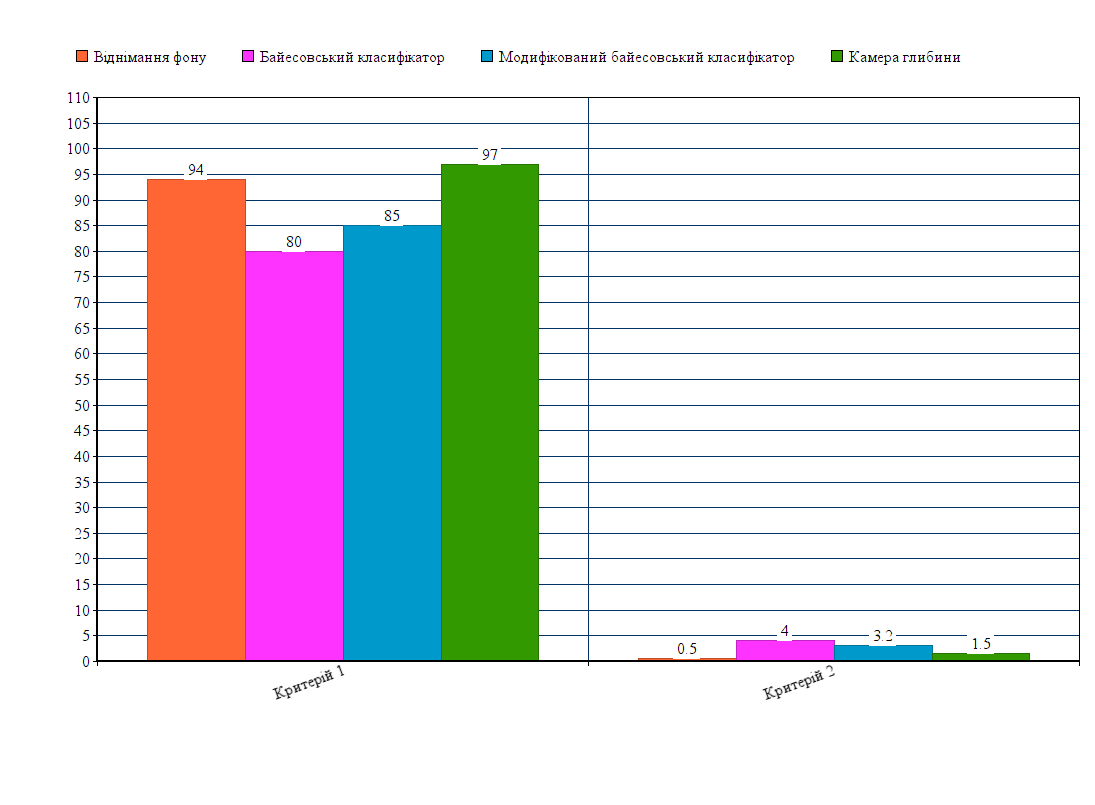
\includegraphics[width=0.85\linewidth]{im/graph}
\end{frame}

\begin{frame}{Порівняння підходів}
	\manimate
	\begin{table}
		\centering
		\resizebox{\linewidth}{!}{
		\begin{tabular}{|l|l|l|}
			\hline
			Підхід                    & Переваги                                                                                                 & Недоліки                                                                                                                                           \\ \hline
			Віднімання фону           & \begin{tabular}[c]{@{}l@{}}Хороша точність - 95\%\\ Відсутність складних обчислень\end{tabular}          & \begin{tabular}[c]{@{}l@{}}Помічає усі рухомі об'єкти\\ Чутливий до змін освітлення\\ Нестійкий до зміни положення камери\end{tabular}             \\ \hline
			Байесовський класифікатор & \begin{tabular}[c]{@{}l@{}}Достатня точність - 85\%\\ Рух камери не впливає на класифікацію\end{tabular} & \begin{tabular}[c]{@{}l@{}}Чутливий до змін освітлення\\ Помічає усі ділянки зі шкірою\end{tabular}                                                \\ \hline
			Камера глибини            & \begin{tabular}[c]{@{}l@{}}Найкраща точність - 97\%\\ Рух камери не впливає на класифікацію\end{tabular} & \begin{tabular}[c]{@{}l@{}}Потрібна спеціальна камера\\ Складні обчислення у разі синхронізації двох відеопотоків\end{tabular} \\ \hline
		\end{tabular}
		}
	\end{table}
\end{frame}

\begin{frame}{Результати роботи}
	\manimate
	Реалізована система по розпізнаванню людської руки із вибором одного з трьох підходів:
	\begin{itemize}
		\item Віднімання фону;
		\item Байесовський класифікатор;
		\item Використання камери глибини.
	\end{itemize}
	Реалізомані окремі модулі навчання байесовського класифікатора:
	\begin{itemize}
		\item Навчання з папки;
		\item Швидке навчання на базі Intel Realsense F200.
	\end{itemize}
\end{frame}